\section{Technique}
\label{sec:technique}

We model configurations as a set of key-value pairs, where
the keys are strings and the values have arbitrary type. This is
a common abstraction offered
by the POSIX system environment, the Java Properties API,
and the Windows registry.


\subsection{Overview}

Figure~\ref{fig:workflow} sketches the high-level workflow of our technique.
Our technique takes as input a Java program and its configuration options.
It first performs a propagation analysis to identify
the affected predicates for each configuration option (Section~\ref{sec:prop}).
After that, our technique \textit{selectively} instruments
the program on the affected predicates. 
To diagnose an error, users run the instrumented program
with the error-revealing inputs and configurations
 to obtain an execution
profile (Section~\ref{sec:profiling}).
Then, our technique uses the obtained execution profile
to identify the behaviorally-deviated predicates and their
responsible options as the root causes (Section~\ref{sec:analysis}).

%The output error report is a ranked list
%of suspicious configuration options that may cause the exhibited problem.

%, linking each configuration
%to its affected predicates

%\ourtool tracks dependencies introduced by both data and
%control flow. It propagates dependencies among xxx


\begin{figure*}[!]
  \centering
  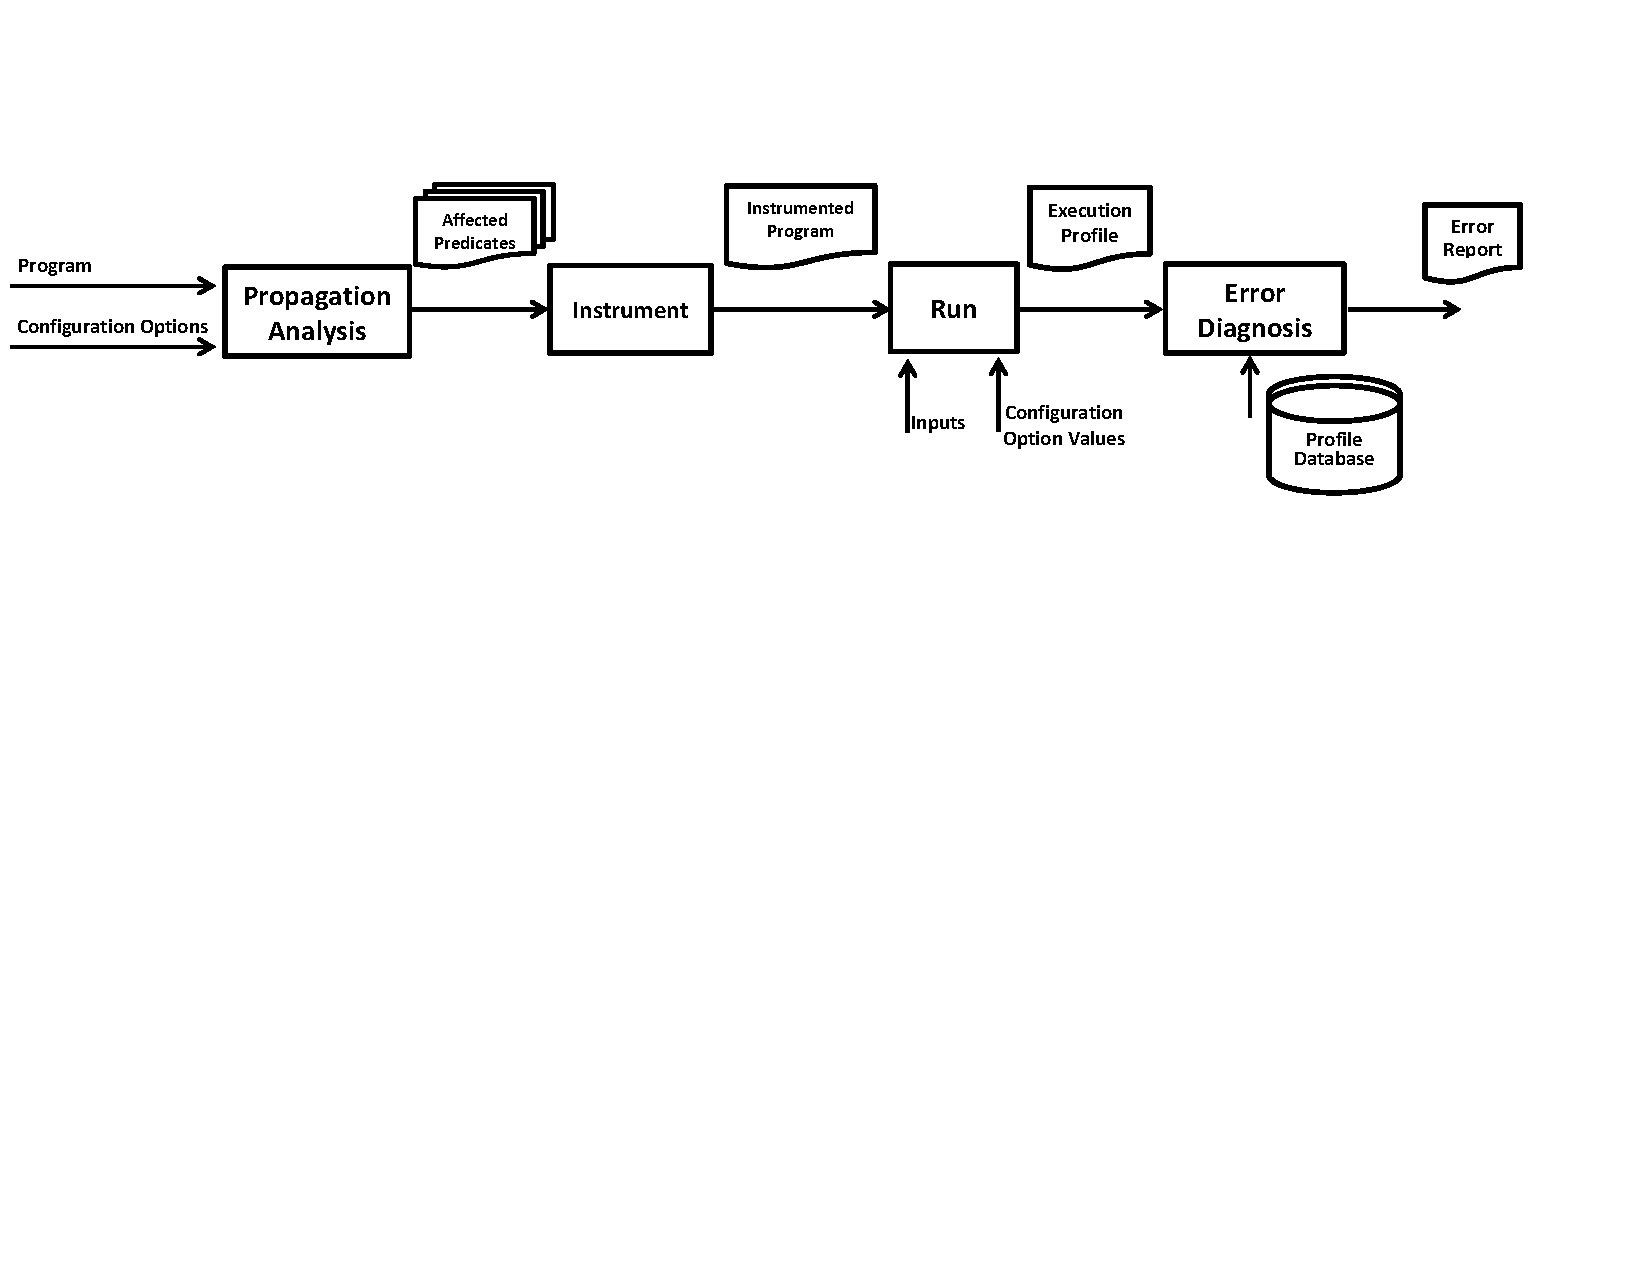
\includegraphics[scale=0.600]{architecture}
  \vspace*{-2.0ex}\caption {{\label{fig:workflow} The workflow of our configuration error diagnosis technique.
Phases ``Instrument'' and ``Run'' correspond to the Configuration Behavior Profiling step in Section~\ref{sec:profiling}.
The other two phases: ``Propagation Analysis'' and ``Deviation Analysis'' correspond to steps in Section~\ref{sec:prop} and Section~\ref{sec:analysis}, respectively.
}}
\end{figure*}

\subsection{Configuration Propagation Analysis}
\label{sec:prop}

For each configuration option, this step statically determines
its affected \textit{predicates}. In our context, a \textit{predicate}
is a boolean expression in a conditional or loop statement, whose evaluation result
decides whether to execute the followed statement or not.
A predicate's rutnime outcome affects the program control flow and could alter
the the program's state consequently. In \ourtool, we focus on identifying and monitoring a program's
control flow instead of an arbitrary data flow based on the
following two observations. First, control flow 
often propagates the majority of configuration-related affects
and is essential to a program's execution path, while
the value of a specific data flow point is largely input-dependent.
And second, the outcome of a program predicate can only be
either true or false; thus, the number of recorded states in monitoring
affected control flow is far less than monitoring arbitrary
data values.  Program predicate is not the only abstraction our technique can use;
however, as we show empirically in Section~\ref{sec:evaluation},
choosing other abstractions such as monitoring statement-level coverage
or method-level invariant yields less accurate results.


To identify predicates affectd by a configuration option, a straightforward
way is using program slicing~\cite{Horwitz:1988} to compute
a forward slice from the initialization statement of a
configuration option. Unfortunately, traditional slicing has
several limitations that prevent it from being directly applicable.
First, traditional slicing does not distinguish flows along
pointers from flows along values; thus, a resulting slice includes all statements that
\textit{may} affect a point of interest and often grows too large. Second,
in our context of configuration error diagnosis,
when having no knowledge of what inputs a software user would provide,
traditional slicing captures every single detail of the execution,
much of which may not be needed at all by pinpointing an incorrect
configuration option value. $\blacksquare$ this second claim needs revising.

Take the code in Figure~\ref{fig:example} as an example to illustrate
this problem.  Tranditional slicing identifies the predicates
in lines 104, 312, and 315 are affected by the configuration option \CodeIn{maxsize}.
However, the predicates in lines 104 and 315, though possibly
affected by the value of \CodeIn{maxsize}, should not be included. $\blacksquare$
In other words, whether a sequence has an active flag (line 104) or
whether a sequence has been executed before (line 315)
is irrelevant with the value of \CodeIn{maxsize}. Monitoring
such predicates and linking their behaviors with the \CodeIn{maxsize}
option may introduce noise and decrease the diagnosis accuracy.

%However, if the provided input changes the workflow,
%instead of all data flow into it. 

To overcome this limitation, our technique uses thin
slicing~\cite{Sridharan:2007} as a manner to include
\textit{only} statements that are \textit{directly} affected by a configuration option.
Differing from traditional slicing, thin slicing
focuses on statements that flow values to the seed (here, a
seed is the initialization statement of a configuration option), ignoring the 
control flow dependencies as well as the uses of
base pointers. Thus, thin slicing improves the relevance
of the slice by only including the statements that compute
and copy a value to the seed.
This property separates
pointer computations from the flow of configuration option value,
naturally connects a configuration option with its
directly affected statements, and makes thin slicing
especially attractive.
For example, in the code excerpt of Figure~\ref{fig:example},
a forward thin slice computed for \CodeIn{maxsize}
only includes the predicate in line 312.
In our experiments (Section~\ref{sec:evaluation}), 
we also empirically compare traditional slicing with
thin slicing in diagnosing configuration errors, and demonstrate
that thin slicing is a better chioce.

%When Randoop is used to generate tests for different inputs (here,
%input mean programs under test), the created tests (method-call
%sequence at line 12) would be dramatically different.
%However, for similar inputs, the program execution flow should
%be similar.


%In fact, there is another configuration option $\blacksquare$
%that affect line 6.

% 

\subsection{Configuration Behavior Profiling}
\label{sec:profiling}

This step instruments the tested program offline
by inserting code to monitor
each the outcome of each affected predicate at runtime.


For the code in Figure~\ref{fig:example} where
the predicate at line 312 is affected by
the configuration option \CodeIn{maxsize}, \ourtool inserts the
following two instrumentation
statements before and after line 312 to count the number of
the predicate being executed and the number being evaluated to true.


\begin{CodeOut}
\begin{alltt}
310. private ExecutableSequence createNewUniqueSequence() \ttlcb
311.   Sequence newSequence = ...; 
       \underline{incrExecCount("maxsize", "newSequence.size() > maxsize");}
312.   if (newSequence.size() > maxsize) \ttlcb
         \underline{incrTrueCount("maxsize", "newSequence.size() > maxsize");}
314.     return null;
      ...
319. \ttrcb
\end{alltt}
\end{CodeOut}


$\blacksquare$The instrumented program expresses an execution
as a trace comprising a vector of \textit{predicate profiles}.
Each predicate profile is a pair of configuration
option and its affected predicate.
The predicate profile also keeps the recorded runtime information.
%of the affected predicate, including
%the count of the predicate being executed and the count of it
%being evaluated to true. 

%\ourtool expresses an execution as
%a predicate profile vector. 
As we
show in the experiments (Section~\ref{sec:evaluation}), such predicate profile
vectors, although by no mean complete, capture
sufficient information to permit users
to reason about the causal effects of configurations
and how they relate to a software's behavior, while
also imposing a moderate amount of performance impact
on foreground applications.


%health as the results of executing a set of predicates.

%As we will show in the experiments~\cite{}, this profile
%provides valuable information about the
%program execution and can help validate a test suite
%or indicate the usage context of a function
%or other computation.

%A software user seeking on specific piece of
%information or aiming to verify a specific invariant
%and uninterested in any other facts about the code
%may be able to use xxx to advantage, but will not
%get as much from it as a programmer open to other,
%possibly valuable information.


\subsection{Configuration Deviation Analysis}
\label{sec:analysis}

\ourtool starts error diagnosis 
after obtaining the execution trace from
an erroneous execution. It first compares it with
existing traces from known correct executions, selects
similar traces for comparison (Section~\ref{sec:similar}),
identifies the most behavioral-deviated predicates
(Section~\ref{sec:deviation}), and then determines
its most likely responsible options (Section~\ref{sec:linking}).


\subsubsection{Selecting Similar Traces for Comparison}
\label{sec:similar}

\ourtool's pre-built database contains a number of
traces from known correct executions, in which one trace
can be dramatically different from another. To
determine how and why the observed trace behaves
differently from the correct ones, \ourtool first
compares and contrasts the 
the erroneous execution with other correct ones, and
then selects a set of similar ones. $\blacksquare$

Given a trace $t$, \ourtool first aggregates
the observed predicate profiles into a $n$-dimensional
vector $v_{t}$ =$\langle r_1, r_2, ..., r_n\rangle$ , where $n$
is the number of predicates in the program and each $r_i$ is
the ratio of the $i$-th predicate profile being evaluated
to true at runtime. If a predicate is not executed in
a particular execution, \ourtool assigns \CodeIn{null} to its true ratio.


When comparing two traces $t_1$ and $t_2$, \ourtool computes
their inner-product distance of the normalized vectors, and selects
those with distance below a threshold (default value: 0.3,
as we used in experiments). When computing the inner-product distance,
if the value of some dimensional is \CodeIn{null}. $\blacksquare$

For crashing errors, \ourtool does not select similar traces.
Instead, it uses all available traces in the database
for comparison, because all traces there are from correct
executions, and can
be served as reference to identify the crashing root causes. $\blacksquare$

\subsubsection{Identifying Deviated Predicates}
\label{sec:deviation}


The comparison between an erroneous trace with a set
of \textit{similar} traces forms a basis for our
automated error diagnosis approach. Given an erroneous trace and a set of similar but correct trace,
the differences in predicate profiles provide evidence for what parts of a program might be
incorrect and why. This helps to further reason about its root cause.


For each observed predicate $p$, \ourtool uses the following metric
to characterize its deviation degree in two traces $t_1$ and $t_2$:

\[
\|Deviation|(p) = |\phi(t_1, p) - \phi(t_2, p)|
\]

\[
\|\phi|(t, p) = \frac{2}{\frac{1}{\|trueRatio|(t, p)} + \frac{1}{totalNum(t, p)}}
\]

$trueRatio(t, p)$ is a function that returns the ratio of predicate $p$ being
evaluated to true in trace $t$, and $totalNum(p)$ is a function
that returns the total number of observations of predicate $p$ in trace $t$..

The metric $\phi$ has some good properties in characterizing the $\blacksquare$

For non-crashing errors, since the obtained trace is a complete one,
\ourtool computes the $Deviation$ metric for each observed predicate in
both traces, and ranks them in a decreasing order based on the computed $Deviation$ value.

For crashing erros, since the obtained trace is incomplete,
\ourtool computes the $Deviation$ metric for the predicates only appearing
in the crashing trace, and ranks them decreasingly based on the computed value.


%\subsubsection{Filtering Execution Noises}
%remove some off-by-one


\subsubsection{Linking Predicates to Root Causes}
\label{sec:linking}

$\blacksquare$

The last step in \ourtool is to link those behavioral-deviated
predicates to its root causes, and rank the suspicious
configuration options as the output.

The intuition behind is that \ourtool determines that
altering a configuration option may change the application�s
control flow such that it deviates from the correct trace,
 it reports that option as a possible root cause.

When comparing an erroneous trace with a set of correc traces,
\ourtool first ranks suspicious configuration options between
each trace pair, and then averages the ranking across traces.

It first identifies the most deviated predicate profile, and
its affecting predicate.
It identifies the configuration option
affecting the highest ranked predicate profile as the most likely
root cause; in the case of ties, it ranks all tied options
based on its distance in a thin slicing SDG.
%as being equally likely to be the root cause.

Finally, needs to average the results


\subsection{Discussions}

We next some design issues in \ourtool.

\vspace{1mm}
\noindent \textbf{Differences between program inputs and configuration options.}
A configurable software system permits users to
customize its behaviors before being used. Broadly speaking,
there is not any fundamental difference between a configuration option
value and a program input value. $\blacksquare$ a configuration option
value is more like a meta-input, which pre-defines the overall expected program
execution details and is usually fixed for a broad range of inputs.
By contrast, an input is more specific for a certain execution $\blacksquare$


\vspace{1mm}
\noindent \textbf{Why cannot use executions from unit tests?}
The pre-built database in \ourtool is designed to contain complete
execution traces, while a unit test that focuses on verifying the
isolated program component behavior in isolation often produces
an incomplete trace. In contrast, a crashing or non-crashing configuration
error from field software application often starts from the main method,
comparing its resulting trace with the partial trace from unit tests
may yield wrong results. $\blacksquare$
%Why cannot use unit test to achieve the trace? since it is incomplete


%why cannot delta debugging? no working state, no predicate

\vspace{1mm}
\noindent \textbf{Why not only store correct traces in the database?}
It is more developers to provide correct executions, instead of
anticipating the possibly error behaviors a user may encounter. $\blacksquare$
A broader question is which kind of informatin should be recorded
from program execution. \ourtool uses predicate as the abstraction level,
and emprically compares with two other abstractions (a coarser abstraction
at the method level, and a finer abstract at the statement level). Investigating
other abstraction levles remains as our future work.

%Why dynamic slicing is not usable? No seed statement, and great overhead. Using JSlicer incurs
%a great overhead. It needs to track every instruction and
%perform synchronization when dependence graph is updated.

%Our technique can be seen as a way to reduce overhead,
%including selective profiling, and static pre-processing
%techniques.

